\clearpage

\def\PRName#1{\textsc{Pre-#1}}

\section{Implementation}

In \cite{Fmaster} a streaming target language for a minimal SNESL was defined.
With trivial changes in the instruction set, this language, named as SVCODE (streaming VCODE), has been implemented on a multicore system in \cite{Fphd}; the various experiment results
have demonstrated single-core performance similar to sequential C code for some simple 
text-processing tasks as well as the
potential for further performance improvment by scheduling opitmization and code analysis.

In this thesis, we put emphasis on the formalization of this low-level language's semantics.
Also, to support recursion in the high-level language at the same time preserving the cost, non-trivial extension of this language is needed. 


\subsection{SVCODE Syntax}
The data or $streams$ that an SVCODE program computes are basically vectors of consts. 
For our minimal language, a primitive stream $\a$ can be a vector of booleans, integers or units, as the following grammar shows:

$$b \in \mathbb{B} = \{\T,\F \}$$
$$ a ::= n \ | \ b \ | \ \unit$$
$$\b = \vrange{b_1}{b_i}$$ 
$$\c = \vrange{()}{()} $$
$$\a = \vrange{a_1}{a_i}  $$ 

\hspace{1cm}

The grammar of SVCODE is given in Figure~\ref{fig-svcode-grammar}.


\begin{figure}[!h] \large
	\begin{alignat*}{2}
	&p  && :: = \ \epsilon \\ 
	& &&\ \ | \ \sdef{\s}{\psi(s_1,...,s_k)}  \tag{$\s \notin \{s_1,...,s_k\}$}\\
	& &&\ \ | \ \withctrl{\s}{p_1}{\Sin}{\Sout}  \tag{$ \FV{p_1} \subseteq \Sin, \Sout \subseteq \dv{p_1} $} \\
	& &&\ \ | \ p_1;p_2  \tag{$\dv{p_1} \cap \dv{p_2} = \emptyset$} \\
	\\
	& \s && ::= 0 \ | \ 1 \ ... \in \SId  = \mathbb{N}   \tag{stream ids}\\
	\\
	& \psi \ && ::= \consta{a} \ | \ \toflag  
	\ | \ \usum \ | \ \maptwo{\oplus} \ | \ \scan_{n_0} \ | \ \distr  \tag{Xducers} \\
	& \oplus \ && :: = + \ | \ - \ | \ \times \ | \ \div \ | \ \% \ | \ \le \ | \ ...  \tag{binary operations}\\
	\\
	&  \S && ::= \{\s_1,..., \s_i\} \in \sset  \tag{a set of stream ids}\\
	\end{alignat*}
\caption{Grammar of SVCODE \label{fig-svcode-grammar}}
\end{figure}

The instructions in SVCODE that perform the computation directly on primitive streams are stream definitions in the form
$$\sdef{\s}{\psi(s_1,...,s_k)} $$  
where $\lcall$ is a primitive function, or a $Xducer$(transducer), taking stream $s_1,...,s_k$ as parameters and returning $s$. 

The only essential control struture in SVCODE is the instruction 
$$\withctrl{\s}{p_1}{\Sin}{\Sout} $$
which may or may not execute a piece of SVCODE program $p_1$, but always defines a bunch of stream variables $\Sout$. Discussions about this \wc 
instruction will occur again and again throughout the thesis as it plays a significant role in dealing with most of the issues we are deeply concerned, 
including cost model correctness and dynamic unfolding of recursive functions. 




The function $\texttt{dv}$ returns the set of defined variables of a given SVCODE program.

\begin{alignat*}{2}
&\dv{\epsilon} && =  \emptyset \\
&\dv{\sdef{\s}{\psi(s_1,...,s_k)}} && =  \{s\} \\
&\dv{\withctrl{\s_c}{p_1}{\Sin}{\Sout}} && =   \Sout \\
&\dv{p_1;p_2} && =  \dv{p_1} \cup \dv{p_2} \\
\end{alignat*}

Correspondingly, $\texttt{fv}$ returns the free variables set.

\begin{alignat*}{2}
&\FV{\epsilon} && = \emptyset \\
&\FV{\sdef{\s}{\psi(s_1,...,s_i)}} && = \{s_1,...,s_k\}\\
&\FV{\withctrl{\s_c}{p_1}{\Sin}{\Sout}} && = \{s_c\} \cup \Sin \\
&\FV{p_1;p_2} && = \FV{p_1} \cup (\FV{p_2} - \dv{p_1}) \\
\end{alignat*}


An immediate property of this language is that the defined variables of a well-formed SVCODE program are always $fresh$. In other words, there is no overlapping between the free variables and the newly generated ones.
\begin{lem}
	$\FV{p} \cap \dv{p} = \emptyset $. 
\end{lem}

The proof is straightward by induction on the syntax of $p$.



\subsection{SVCODE semantics}

Before showing the semantics, we first introduce some notations and operations about streams for convenience.
\begin{nota}
	Let $\< a_0 | \a \'>$ denote a non-empty stream $\< a_0,a_1,...,a_i \'>$ for some $\a = \< a_1,...,a_i \'>$. 
\end{nota}


\begin{nota}[\textbf{Stream concatenation}]
$\vapp{\vrange{a_1}{a_i}} {\vrange{a_1'}{a_j'}} = \langle a_1,...,a_i,a_1',...,a_j' \rangle $ \\
	
\end{nota}

The operational semantics of SVCODE is given in Figure~\ref{fig-svcode-semantics}.
The runtime environment or store $\sgm$ is a map from stream variables to vectors:
 $$\sgm = [\s_1 \|-> {\a_1},...,\s_i \|-> {\a_i}]$$
The $control \ stream$ $\c$, which is basically a vector of units representing an unary number, indicates the $parallel \ degree$ of the computation. The role of control stream will become much clearer when we come to the semantics of Xducers. It is worth noting that only in the rule $\PName{Wc-Nonemp}$ the control stream has a chance to get changed.

	
\begin{figure}[!h]\large 

\Jug{\seval{p}{\sgm}{\c}{\sgm'}}\\


\PT{\LeLa{\PName{Empty:}}  \Axiom{{\seval{\epsilon}{\sgm}{\c}{\sgm}}{}}} \\[2ex]

\PRule{Xducer}{\PT{\AC{\sevalf{\a_1}{\a_k}{\c}{\a}}
	\RiLa{((\sgm(\s_i) = \a_i)^k_{i=1})}
	\UC{\seval{\sdef{\s}{\lcall\Tupk\s}}{\sgm}{\c}{\sgm[\s \|-> \a]}}
}} \\[4ex]

\PT{ \LeLa{\PName{Wc-Emp:}}
	\AC{}
	\RiLa{
		\left(
			\begin{aligned}
				&\forall s \in \{s_c\} \cup \Sin. \sgm(s) = \emptyv \\
				&\Sout = \{s_1,...,s_l\}
			\end{aligned}
		\right)}
	\UC{\seval{\withctrl{\s_c}{p_1}{\Sin}{\Sout}}{\sgm}{\c}{\sgm[\l{\s_i \|-> \emptyv}]}}
}\\[2ex]
\PRule{Wc-Nonemp}{\PT{
	\AC{\seval{p_1}{\sgm}{\c_1}{\sgm''}}
	\RiLa{\left(
		\begin{aligned} 
		&\sgm(\s_c)= \c_1 \ne \emptyv \\
	    &\Sout = \{s_1,...,s_l\}
		\end{aligned}\right)}
	\UC{\seval{\withctrl{\s_c}{p_1}{\Sin}{\Sout}}{\sgm}{\c}{\sgm[\l{\s_i \|-> \sgm''(\s_i)}]}}
}}\\[4ex]

\PRule{Seq}{\PT{
	\AC{\seval{p_1}{\sgm}{\c}{\sgm''}}
    \AC{\seval{p_2}{\sgm''}{\c}{\sgm'}}	
    \BC{\seval{p_1;p_2}{\sgm}{\c}{\sgm'}}
}}

\caption{SVCODE semantics}
\label{fig-svcode-semantics}
\end{figure}

The rule $\PName{Empty}$ is trivial, empty program doing nothing on the store. 

The rule $\PName{Xducer}$ adds the store a new stream binding where the bound vector is generated by a specific Xducer with input streams. The detailed semantics of Xducers are defined in the next subsection. 

The rules $\PName{Wc-Emp}$ and $\PName{Wc-Nonemp}$ together show two possibilities for interpreting a \wc instruction:
\begin{itemize}
	\item if the new control stream $\s_c$ as well as the streams in $\Sin$, which includes the free variables of $p_1$, are all empty, then just bind empty vectors to the streams in $\Sout$, which are part of the defined streams of $p_1$.
	\item otherwise execute the code of $p_1$ as usual under the new control stream, ending in the store $\sgm''$; then copy the bindings of $\Sout$ from $\sgm''$ to the initial store. 
\end{itemize}
The new control stream is crucial here, because it decides whether or not to execute $p_1$, which is the key to avoiding infinite unfolding of recursive funtions. For an eager interpreter of SVCODE, if we count one stream definition as one step, then this skip guarantees the low-level step cost agrees on the high-level one. Also, skipping a certain piece of code should help improve the efficiency of execution.



\subsection{Xducers}

\subsubsection{SVCODE Dataflow}
Transducers or $Xducers$ are the primitive computing functions on streams in SVCODE. Each Xducer consumes a number of streams and transforms them into another. 

As we can see from the side condition of the rule $\PName{Xducer}$, a stream can be consumed only after it has been produced.
Thus, the dataflow among an SVCODE program constructs a DAG (directed acyclic graph), where each Xducer performs one node. 
Figure~\ref{fig-svcode-eg1} shows an example program with its DAG in Figure~\ref{fig-svcode-dag1}. \\

\begin{figure}[h]
	\begin{lstlisting}[style=svcode-style]
	S1 := Const_3();
	S2 := ToFlags(S1);
	S3 := Usum(S2);
	[S4] := WithCtrl(S3,[], S4 := Const_1();)
	S5 := ScanPlus(S2, S4);
	\end{lstlisting}	
\caption{A small SVCODE program \label{fig-svcode-eg1}}
\end{figure}
	
\hspace{1cm}

\fig{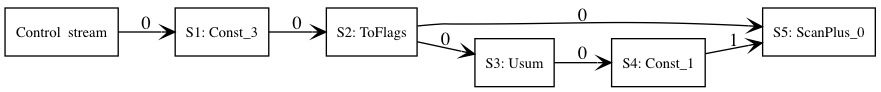
\includegraphics[width=1.1\textwidth]{fig/xducerDag2.png}}{
Dataflow DAG for the code in Figure~\ref{fig-svcode-eg1}.
\label{fig-svcode-dag1}
Note that, for simplicity, the control stream is added as an explicit supplier only to Xducer $\consta{a}$.
}


When we talk about two Xducers $A$ and $B$ connected by an arrow from $A$ to $B$ in the DAG, we call $A$ a $producer$ or a $supplier$ to $B$, and $B$ a $consumer$ or a $client$ of $A$. 
As an Xducer can have multiple suppliers, we distinguish these suppliers by giving each of them an index, called a $channel \ number$. 
In Figure~\ref{fig-svcode-dag1}, the channel number is labeled above each edge. 
For example, the Xducer S2 has two clients, S3 and S5, for both of whom it is the No.0 channel;  Xducer S5 has two suppliers: S2 the No.0 channel and S3 the No.1. 


\subsubsection{General semantics}
The semantics of Xducers are abstracted into two levels: the $general$ level and the $block$ level. The general level summarizes the comman property that all Xducers share, and the block level describes the specific behavior of each Xducer. 

Figure~\ref{fig-xducer-semantics} shows the semantics at the general level. 


\begin{figure}[h]\large
	
	\Jug{\sevalf{\a_1}{\a_k}{\c}{\a}} \\
	
	
	\PRule{X-Loop}{\PT{
			\AC{\block{\a_{11}}{\a_{k1}}{\a_{01}}}
			\AC{\sevalf{\a_{12}}{\a_{k2}}{\c_0}{\a_{02}}}
			\RiLa{((\vapp{\a_{i1}}{\a_{i2} = \a_i})^k_{i=0})}
			\BC{\sevalf{\a_1}{\a_k}{\< () | \c_0 \rangle}{\a_0}}
	}}\\[4ex]
	
	\LeLa{\PName{X-Termi:}} 
	\Axiom{\sevalf {\emptyv_1} {\emptyv_k} \emptyv \emptyv}
	\DisplayProof \footnotemark	
	\caption{Semantics of SVCODE transducers \label{fig-xducer-semantics}}
\end{figure}
\footnotetext{For notational convenience, in this thesis we add subscripts to a sequence of constants, such as $\emptyv, \F, 1$, to denote the total number of these constants.}

There are only two rules for the general semantics. 
They together say that the output stream is computed in a ``loop" fashion, where the 
iteration uses specific block semantics of the Xducer and the number of iteration is the unary number that the control stream represents, i.e., the length of the control stream. 
In the parallel setting, we prefer to call this iteration a $block$. 
Recall the control stream is a representation of the parallel degree of the computation, then a block consumes exact one degree. 
We note that all these blocks are data-independent, which means they can be performed in parallel. 
Now it is clear that the control stream indeed carrys the theoretical
maximum number of processors we need to execute the computation most efficiently (if the computation within the block can not be parallelized further)(???).



\subsubsection{Block semantics}
After abstracting the general semantics, the remaining work of formalizing the specific semantics of Xducers within a block becomes relatively clear and easy. The block semantics are defined in Figure~\ref{fig:xducer-bl-seman}. 

\fig{
	\def\'>{\rangle}
	
	\Jug{\block{\a_1}{\a_k}{\a}} \\
	
	\PT{\LeLa{\PName{Const:}} 
		\Axiom{\blockf{\consta{a}}{}{\singl{a}}}
	}
	\PT{\LeLa{\PName{ToFlags:}} 
		\Axiom{\blockf{\toflag}{\singl{n}}{\< \F_1,...,\F_n,\T \'>}} } \\[4ex]
	
	\PRule{MapTwo}{\PT{\AC{}
			\RiLa{(n_3= n_1 \oplus n_2)}
			\UC{\blockf{\maptwo{\oplus}}{\singl{n_1}, \singl{n_2}} {\singl{n_3}}}
	}} \\[4ex]
	
	%--- UsumF
	\PRule{UsumF}{
		\PT{\AC{\blockf{\usum}{\b}{\a}}
			\UC{\blockf{\usum}{ \<\F|\b \'>}{\<()|\a\'>}}
		}
	}
	\PT{\LeLa{\PName{UsumT:}} \Axiom{\blockf{\usum}{\oT}{\emptyv}}}
	\\[4ex]
	
	\PRule{ScanF}{
		\PT{\AC{\blockf{\scan_{n_0+n}}{\b,\a}{\a'}}
			\UC{\blockf{\scan_{n_0}}{\<\F|\b \'>, \<n|\a\'>}{\<n_0|\a'\'>}}
		}		
	}
	\PT{\LeLa{\PName{ScanT:}} \Axiom{\blockf{\scan_{n_0}}{\oT, \emptyv}{\emptyv}}}\\[4ex]
	
	
	\PRule{DistrF}{
		\PT{\AC{\blockf{\distr}{\b, \<n\'>}{\a}}
			\UC{\blockf{\distr}{\<\F|\b \'>, \<n\'>}{\<n|\a \'>}}
		}
	}
	\PT{\LeLa{\PName{DistrT:}}\Axiom{\blockf{\distr}{\oT,\<n\'>}{\emptyv}}}\\[1ex]
}{Semantics of transducer blocks \label{fig:xducer-bl-seman}}



\begin{itemize}
\renewcommand{\labelitemi}{$-$}
	\item $\constaf{a}$ outputs the const $a$ until the control stream reaches EOS.
	
	\begin{example} \emph{$\constaf{3}$ with control stream $\c = \<(),()\'>$:}\\
	\begin{center}
		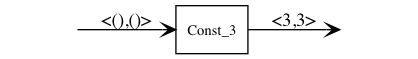
\includegraphics[width=0.6\textwidth]{fig/const3.png}
	\end{center}
	\end{example}

	\item $\toflagf{\singl{n}}$ first outputs $n$ $\F$s, then one $\T$.
	
	\begin{example} \emph{$\toflagf{\<2,0\'>}$:}\\
		\begin{center}
		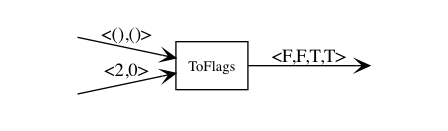
\includegraphics[width=0.6\textwidth]{fig/toflag.png}
		\end{center}
	\end{example}
	
	\item $\maptwof{\oplus}{\singl{n_1}}{\singl{n_2}}$ outputs 
	the binary operating result of $\oplus$ on $n_1$ with $n_2$. 

	\begin{example} \emph{$\maptwof{+}{\<3,2\'>}{\<1,1\'>}$:}\\
		\begin{center}
			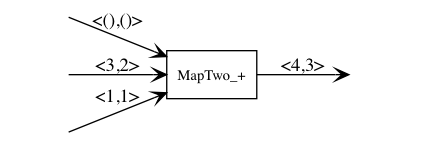
\includegraphics[width=0.6\textwidth]{fig/maptwo.png}
		\end{center}
	\end{example}
	
	\item $\usumf{\b}$ transforms an $\F$ to a unit, or a $\T$ to nothing. It is the only Xducer that can generate a unit vector,
	so it is mainly used when we need to replace the control stream.
	\begin{example} \emph{$\usumf{\<\F,\T,\F,\F,\T\'>}$:}\\
		\begin{center}
			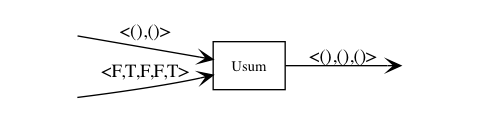
\includegraphics[width=0.6\textwidth]{fig/usum.png}
		\end{center}
	\end{example}
	
	\item $\scan_{n_0}(\b,\a)$ performs an exclusive scan of the binary operation plus on $\a$, segmented by $\b$, with a starting element $n_0$.
		\begin{example} \emph{$\scan_{0}(\<\F,\F,\F,\T,\F,\T\'>, \< 2,5,3,6 \'>)$}\\
		\begin{center}
			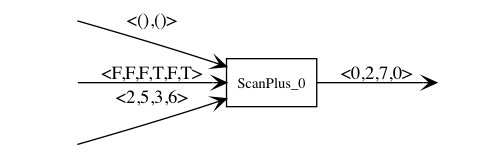
\includegraphics[width=0.7\textwidth]{fig/scan.png}
		\end{center}
	\end{example}
	 
	\item $\distr(\b,{\singl{n}})$ replictes the const $n$ $u$ times where $u$ is the unary number segmented by $b$. 
	\begin{example} \emph{$\distrf{\<\F,\F,\F,\T,\F,\T\'>}{\< 2,5 \'>}$}\\
		\begin{center}
			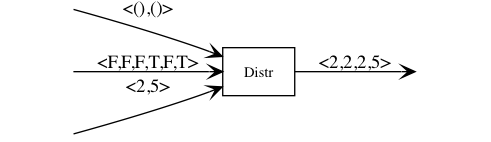
\includegraphics[width=0.7\textwidth]{fig/distr.png}
		\end{center}
	\end{example}
	
\end{itemize}

		


As we have discussed before, we consider a block  as the minimum computing unit assigned to a single processor. This is reasonable for
Xducers such as $\consta{a}$ and $\maptwo{\oplus}$, because
they are already sequential at the block level. 

However, some other Xducers, such as $\usum$, can be parallelized further inside a block.
As we extend the language with more Xducers, we could find that computations on unary numbers within blocks are common, which is mainly due to the value represenation strategy we use, but also more difficult to be regularized.
For the scope of this thesis, the block semantics we have shown are already relatively clear and simple enough to reason about, and the unary level parallelism can be investegated in future work. 
 
 

%Or if we want to use $unary$ semantics maybe for later: \\
%\begin{mdframed}
%\PT{
%	\AC{\unary{\singl \F}{\a_{k1}}{\a_1}}
%	\AC{\block{\a_{12}}{\a_{k2}}{\a_2}}
%	\RiLa{(\a = \vapp{\a_1}{\a_2})}
%	\BC{\block{\vapp {\singl\F} {\a_{12}}} {\vapp {\a_{k1}} {\a_{k2}}}{\a}}
%}\\[2ex]
%
%\PT{
%	\AC{\unary{\oT} {\a_k}{\a}}
%	\UC{\block{\oT}{\a_k} \a}
%}\\[2ex]
%
%\begin{itemize}
%\item Transducer $unary$ semantics:\\ 
%
%\Jug{\unary{\singl b}{\a_k}{\a}}
%
%\PT{ \Axiom{\usum(\oF) \dda \vunit}}
%\PT{\Axiom{\usum(\oT) \dda \emptyv }} \\[1ex]
%
%
%%loopuv
%\item Transducer block with $accumulator$: \\
%
%\Jug{\blockv{n}{\a_1}{\a_k}{\a}}
%\PT{
%	\AC{\unaryv{n_0} {\singl \F}{\a_{k1}}{n_0'} {\singl{n_1}}  }
%	\AC{\blockv{n_0'}{\a_{12}}{\a_{k2}}{\a_2}}
%	\BC{\blockv{n_0} {\vapp {\singl\F} {\a_{12}}} {\vapp {\a_{k1}} {\a_{k2}}}{\vapp {\singl{n_1}} {\a_2}} }
%}\\[2ex]
%
%\PT{
%	\AC{\unaryv {n_0} \oT {\a_k} {} {\a}}
%	\UC{\blockv {n_0} \oT {\a_k} {\a} }
%}
%
%\item Transducer unary with $accumulator$: \\
%
%\Jug{\unaryv{n}{\oF}{\a_k}{n'}{\a}}
%
%\PT{\Axiom{\scan_{n_0}(\oF,{\singl{n}}) \dda^{n_0+n} {\singl{n_0}} }} \\
%
%\Jug{\unaryv{n}{\oT}{\a_k}{}{\a}}
%
%\PT{\Axiom{\scan_{n_0}(\oT, \emptyv) \dda {\emptyv} }}
%\end{itemize}
%\end{mdframed}

%
%\subsubsection{Data consuming rate}
%
%Because the data from different channels are usually not only different
%types, but also different consuming rate -- the number of constant that
%the Xducer consumes at each



\subsection{SVCODE determinism}

As we have given formal semantics to the language, we now argue that a well-formed SVCODE program is deterministic.

 
\begin{defi}[\textbf{Stream prefix}]
	$\a$ is a $prefix$ of $\a'$, written $\a \prefix \a'$, if one the following rules applys: \\
	
	\emph{\Jug{\a \prefix \a'}}
	\PT{\LeLa{\PRName{Emp:}} \Axiom{\emptyv \prefix \a' }}
	\PRName{Nonemp:}{
		\PT{
			\AC{\a \prefix \a'}
			\UC{\<a_0 | \a \'> \prefix \<a_0 | \a' \'>}
		}}
	
\end{defi}

\begin{lem}\label{lem-app2pre}
	If $\a_1 {\++} \a_2 = \a$, then $\a_1 \prefix \a$.
\end{lem}
\begin{proof}
	The proof is straightforward by induction on $\a_1$: case $\a_1 = \emptyv$ and case $ \a_1 = \< a_0, \a_1' \'>$ for some $\a_1'$.
\end{proof}

One may notice that in the rule $\PName{X-Termi}$ both the control stream and the parameter stream(s) must be all empty, and no rules apply to the other cases where one of them is empty while the other is not. The following lemma explains why the other cases can never happen: 
there is only one way to cut down a prefix of each input stream for
a specific Xducer to be consumed in a block.


\begin{lem} \label{lem-block-unique}
	If
	\begin{enumerate}[(i)]
		\item $(\a_i' \prefix  \a_i \ by \ some \ derivation \ \MP_{ri})^k_{i=1}$ and $\block{\a_1'}{\a_k'}{\a'}$ by some $\MP$, 
		\item $(\a_i'' \prefix \a_i \ by \ some \ derivation \ \MP'_{ri})^k_{i=1}$ and
		$\block{\a_1''}{\a_k''}{\a''}$ by some $\MP'$.
	\end{enumerate} 
	then \begin{enumerate}[(i)]
		\item $(\a_i' = \a_i'')^k_{i=1}$ 
		\item $\a' = \a''$.
	\end{enumerate}
\end{lem}

\begin{proof}
	The proof is by induction on the syntax of $\lcall$. We show two cases $\toflag$ and $\scan_{n_0}$ here; the others are analogous.
	\begin{itemize}
	  \item Case $\lcall = \toflag$. \\
	  
		Since there is only one rule for $\toflag$, we must have
		$$	\PT{\LeLa{\MP =} 
			\Axiom{\blockf{\toflag}{\singl{n_1}}{\< \F_1,...,\F_{n_1},\T \'>}} }
		$$
		and 
			$$	\PT{\LeLa{\MP' =} 
			\Axiom{\blockf{\toflag}{\singl{n_2}}{\< \F_1,...,\F_{n_2},\T \'>}} }
		$$
		so $k=1, \a_1' = \singl{n_1}$, $\a' = \< \F_1,...,\F_{n_1},\T \'>$, and  
	     $\a_1'' = \singl{n_2}$, $\a'' = \< \F_1,...,\F_{n_2},\T \'>$. \\
		Since both $\a_1'$ and $\a_1''$ are nonempty, $\MP_{r1}$ and $\MP_{r1}'$ must all use the rule $\PRName{Nonemp}$,
		which implies $n_1$ = $n_2$. 
		Then it is clear that $\a_1' = \a_1''$ and $\a' = \a''$ as required. 

	  \item Case $\lcall = \scan_{n_0}$. \\
	  From the two rules $\PName{ScanT}$ and $\PName{ScanF}$, it is clear that $k$=2, and both $\a_1'$ and $\a''_1$ must be nonempty, which means $\MP_{r1}$ and $\MP_{r1}'$ must all use $\PRName{Nonemp}$. \\
	  By induction on $\a_1$, there are two subcases:
	  \begin{itemize}
	  	\item Subcase $\a_1 = \< \T | \a_{10} \'>$. \\
	  	By $\PRName{Nonemp}$ we know $\a_1'$ and $\a_1''$ must start with a $\T$, thus both $\MP$ and $\MP'$ must use $\PName{ScanT}$, and they must be identical:
	  	$$
	  	  \PT{\LeLa{\MP = \MP' = } \Axiom{\blockf{\scan_{n_0}}{\oT, \emptyv}{\emptyv}}}$$
	  	 So immediately we have $\a'_{1} = \a_1'' = \oT$, $\a_2' = \a_2'' = \emptyv$,
	  	 and $\a' = \a'' = \emptyv$ as required.
	  	
	  	\item Subcase $\a_1 = \< \F | \a_{10} \'>$. \\
	  	By $\PRName{Nonemp}$ we know $\a_1'$ and $\a_1''$ must start with an $\F$, therefore both $\MP$ and $\MP'$ must use $\PName{ScanF}$. 
	  	Assume $\a_2 = \<n | \a_{20} \'>$, then we must have
	  	
	  	$$\PT{\UCN{\MP_0}{\blockf{\scan_{n_0+n}}{\a'_{10},\a'_{20}}{\a_0'}}
	  		\LeLa{\MP = }
	  		\UC{\blockf{\scan_{n_0}}{\<\F|\a'_{10} \'>, \<n|\a'_{20}\'>}{\<n_0|\a'_0\'>}}
	  	}$$
  	    where \eq{eq-scan-determ-1}{
  	    ( \a_{i0}' \prefix \a_{i0} )^2_{i=1}}
  	
  	    So $\a_1' =  \<\F|\a'_{10} \'>, \a_2' = \<n|\a'_{20}\'>$,
  	    and $\a' = \<n_0|\a'_0\'>$.
  	    
  	    Similarly, 
  	    
  	    	$$\PT{\UCN{\MP_0'}{\blockf{\scan_{n_0+n}}{\a''_{10},\a''_{20}}{\a''_0}}
  	    	\LeLa{\MP' = }
  	    	\UC{\blockf{\scan_{n_0}}{\<\F|\a''_{10} \'>, \<n|\a''_{20}\'>}{\<n_0|\a''_0\'>}}
  	    }$$
  	    where  \eq{eq-scan-determ-2}{
  	    	(\a''_{i0} \prefix \a_{i0} )^2_{i=1}}
      	
      	
      	and $\a_1'' =  \<\F|\a''_{10} \'>, \a_2'' = \<n|\a''_{20}\'>$, $\a'' = \<n_0|\a''_0\'>$.
      	
      	By IH on $\eqref{eq-scan-determ-1}$ with $\MP_0$, 
      	$\eqref{eq-scan-determ-2}$, $\MP_0'$, we get
      	$(\a'_{i0} = \a''_{i0})^2_{i=1}$, and $\a'_0 = \a''_0$. \\
      	Thus $\< \F |\a'_{10} \'> = \<\F | \a''_{10} \'>$, i.e., $\a'_1 = \a''_1$. 
      	Likewise, $\a'_2 = \<n|\a'_{20}\'> = \<n|\a''_{20}\'> = \a''_2$, and  $\a' = \<n_0|\a'_0\'> = \<n_0|\a''_0\'> = \a''$ as required. 
	  	
	  \end{itemize}
	
	\end{itemize}
\end{proof}


\begin{lem}[\textbf{Xducer determinism}] \label{lem-xducer-determ}
	If $\sevalfg{\lcall}{\replc{k}{\a}}{\c}{\a_0}$ by some derivation $\MP$,
	and $\sevalfg{\lcall}{\replc{k}{\a}}{\c}{\a'_0}$ by some derivation $\MP'$,
	then $\a_0 = \a'_0$.
\end{lem}

\begin{proof}
	The proof is by induction on the structure of $\c$. There are two cases: $\c = \emptyv$ and $\c = \< () | \c_0 \'>$ for some $\c_0$. The first case is trivial, so we just show the second here.
	\begin{itemize}
		\item Case $\c = \< () | \c_0 \'>$. \\		
		$\MP$ must use $\PName{X-Loop}$:
		$$\PT{
			\UCN{\MP_1}{\block{\a_{11}}{\a_{k1}}{\a_{01}}}
			\UCN{\MP_2}{\sevalf{\a_{12}}{\a_{k2}}{\c_0}{\a_{02}}}
			\LeLa{\MP = }
			\BC{\sevalf{\a_1}{\a_k}{\< () | \c_0 \rangle}{\a_0}}
		}$$
		where 
		\eq{eq-xdu-1}{(\vapp{\a_{i1}}{\a_{i2}} = \a_i)^k_{i=1}}
		\eq{eq-xdu-2}{\vapp{\a_{01}}{\a_{02}} = \a_0}
		Similarly,
			$$\PT{
			\UCN{\MP'_1}{\block{\a'_{11}}{\a'_{k1}}{\a'_{01}}}
			\UCN{\MP'_2}{\sevalf{\a'_{12}}{\a'_{k2}}{\c_0}{\a'_{02}}}
			\LeLa{\MP' = }
			\BC{\sevalf{\a_1}{\a_k}{\< () | \c_0 \rangle}{\a'_0}}
		}$$
		where
		\eq{eq-xdu-3}{(\vapp{\a'_{i1}}{\a'_{i2}} = \a_i)^k_{i=1}}
		\eq{eq-xdu-4}{\vapp{\a'_{01}}{\a'_{02}} = \a'_0}
		
		Using Lemma~\ref{lem-app2pre} $k$ times on \eqref{eq-xdu-1}, we have 
		\eq{eq-xdu-5}{(\a_{i1} \prefix \a_i)^k_{i=1}}
		Analogously, from  \eqref{eq-xdu-3},
		  \eq{eq-xdu-6}{(\a'_{i1} \prefix \a_i)^k_{i=1}}
		
		By Lemma~\ref{lem-block-unique} on \eqref{eq-xdu-5} with
		$\MP_1$, \eqref{eq-xdu-6}, $\MP_1'$, we get
		\eq{eq-xdu-7}{\k{\a_{i1} = \a'_{i1}}}
		\eq{eq-xdu-8}{\a_{01} = \a'_{01}}
		
		It is easy to show that from \eqref{eq-xdu-1}, \eqref{eq-xdu-3} and \eqref{eq-xdu-7} we can get
				\eq{eq-xdu-9}{\k{\a_{i2} = \a'_{i2}}}
		Then by IH on $\MP_2$ with $\MP_2'$, we obtain $\a_{02} = \a'_{02}.$
		
		Therefore, with \eqref{eq-xdu-2}, \eqref{eq-xdu-4}, \eqref{eq-xdu-8}, 
		we obtain $\a_0 = \a_{01} {\++} \a_{02} = \a'_{01} {\++} \a'_{02} = \a'_0$, as required.
	\end{itemize}
	
	 
\end{proof}


\begin{thm}[\textbf{SVCODE determinism}] \label{thm-svcode-determ}
	If $\seval{p}{\sgm}{\c}{\sgm'}$ (by some derivation $\MP$) and $\seval{p}{\sgm}{\c}{\sgm''}$ (by some derivation $\MP'$), 
	then $\sgm' = \sgm''$.
\end{thm}

\begin{proof}
	The proof is by induction on the syntax of $p$. There are four cases: the case for $p = \epsilon$ is trivial; with the help of Lemma~\ref{lem-xducer-determ}, the case for $p = \sdef{s}{\lcall(s_1,...,s_k)}$ is also trivial; proof of $p = p_1; p_2$ can be done by IH; the only interesting case is $p = \withctrl{\s_c}{p_1}{\Sin}{\Sout}$.
	\begin{itemize}
		\item Case $p = \withctrl{\s_c}{p_1}{\Sin}{\Sout}$. \\
		Assume $\Sout = \{s_1,...,s_l\}$. There are two subcases by induction on $\sgm(\s_c)$: 
		\begin{itemize}
			\item Subcase $\sgm(\s_c) = \emptyv$. \\
			Then $\MP$ and $\MP'$ must all use $\PName{Wc-Emp}$, and they must be identical:		
			$$\PT{ 
				\LeLa{\MP= \MP' =}
				\Axiom{\seval{\withctrl{\s_c}{p_1}{\Sin}{\Sout}}{\sgm}{\c}{\sgm[\l{\s_i \|-> \emptyv}]}}
			}$$
		    with $ \forall s \in \Sin. \sgm(s) = \emptyv$.
		    So $\sgm' = \sgm'' = \sgm[\l{\s_i \|-> \emptyv}]$, as required. 
		    
		    \item Subcase $\sgm(\s_c) \neq \emptyv$. \\
		    Then we must have
			$$\PT{
				\UCN{\MP_1}{\seval{p_1}{\sgm}{\c_1}{\sgm_1}}
				\LeLa{\MP = }
				\UC{\seval{\withctrl{\s_c}{p_1}{\Sin}{\Sout}}{\sgm}{\c}{\sgm[\l{\s_i \|-> \sgm_1(\s_i)}]}}
			}$$
		
			Also, we have
			$$\PT{
				\UCN{\MP'_1}{\seval{p_1}{\sgm}{\c_1}{\sgm'_1}}
				\LeLa{\MP' = }
				\UC{\seval{\withctrl{\s_c}{p_1}{\Sin}{\Sout}}{\sgm}{\c}{\sgm[\l{\s_i \|-> \sgm'_1(\s_i)}]}}
			}$$
		
			So $\sgm' = \sgm[\l{\s_i \|-> \sgm_1(\s_i)}]$, 
			and $\sgm'' = \sgm[\l{\s_i \|-> \sgm'_1(\s_i)}]$. \\
			By IH on $\MP_1$ and $\MP'_1$, we obtain
			$$\sgm_1 = \sgm_1'$$
			Then it is clear that $\sgm' = \sgm''$, as required.
			
		\end{itemize} 
		
	\end{itemize}

\end{proof}


\subsection{Streaming interpreter}

\subsection{Recursion}



